
%***********************************************************************

% This is a template to be used for the preparation of
% papers submitted to the 30th International Workshop on
% Statistical Modelling, to be held in Linz, Austria,
% July 6-10, 2015.

% Please follow the following general guidelines:
%
% (1) Do not specify any definitions, commands or style parameters.
%     Upon submission, your file will be checked for presence of
%     \newcommand or \def statements and if found, error message will be reported
%     by the submission form.
%
% (2) Follow the template below very tightly.
%
% (3) Include .pdf figures using the \includegraphics
%      command, an example of which are given below.
%
% (4) Use file names which begin with the surname of the first author.
%
% (5) When creating labels for cross-references, please start always
%     by surname of the first author, e.g., \label{smith:likelihood}
%
% (6) The template below contains some example materials
%      to guide you through the preparation of your paper.  However,
%      remove all the redundant material from your final document
%      before submitting.

% The guidelines above are needed in order to be able to combine all
% the papers into a single proceedings book of acceptable quality.
% Please follow the guidelines as strictly as possible. Deviations may
% result in papers being either refused by the registration form
% or sent back to the authors with the request to change
% their documents according to the guidelines.

% Special characters:
% Please do not use special characters (e.g., accents).
% Use TeX composition instead, such as \~n, \'a, \`e, \v{s}, \r{u} etc.

% Changes as of IWSM 2013:
%  * \usepackage{booktabs} added which allows \toprule et al. in the tabular environment
%    (\hline\hline is not longer used)
%  * '^\T' added in iwsm.sty to denote transposed vectors and matrices within math (see example below)
%  * \usepackage{amsmath, amssymb} introduced since IWSM 2012 is allowed (allowing usage of boldsymbols
%    and other handy constructions (align, pmatrix etc.) within math)
%  * \usepackage{psfrag} introduced since IWSM 2012 is NOT allowed
%
%

%***********************************************************************
% PLEASE LEAVE THIS PART UNCHANGED
%***********************************************************************

\documentclass[twoside]{report}
\usepackage{iwsm}
\usepackage{graphicx}
\usepackage{amsmath, amssymb}
\usepackage{booktabs}
\usepackage{color} % % % %remove before final submission!!!!

% Please do not specify any new definitions, any new commands,
% and do not specify any style parameters.
% The preamble of the document should be left unchanged.

\begin{document}

%***********************************************************************
% PLEASE INSERT YOUR CONTENT FROM HERE
%***********************************************************************

% Title and running title to be used as left header:
%\title{Exploring LD decay with quantiles -- a case study}
\title{Quantifying LD decay by quantile regression -- a case study} 
\titlerunning{Quantiles for LD decay}

% Authors and running list of authors to be used as right header:
\author{Sabine K. Schnabel\inst{1}, Federico Torretta\inst{2} and Matthias Westhues \inst{3}}
\authorrunning{Schnabel et al.}    %% use \authorrunning{Surname 1} if only 1 author
                                    %% use \authorrunning{Surname 1 and Surname2} if two authors
                                    %% use \authorrunning{Surname 1 et al.} if more than two authors

% Institutes of all authors
% Include city and country of each institute, do not include the full address.
\institute{Biometris, Wageningen University and Research Centre,
The Netherlands \and Universit\`a di Palermo, Italy \and Universit\"at Hohenheim, Germany}

% E-mail of presenting author for correspondence
\email{sabine.schnabel@wur.nl}

% Brief abstract of the paper:
\abstract{Still missing.}

% Keywords (at most 5):
\keywords{Quantile regression; smoothing; monotonicity; linkage; LD decay}

% Produce the title:
\maketitle

%***********************************************************************

% Sections and subsections (do not use lower levels):


\section{Introduction and Motivation}

\textcolor{green}{general comment}\newline
\textcolor{blue}{comment to Federico}\newline
\textcolor{red}{comment to Matthias}\newline

Through decreasing costs more and more genotyping data is available in projects in 
biology and agriculture. More genetic markers can be created which results in more 
information on the genetic structure being at the disposure of the investigators. However, 
more available data does not forcedly result in more information available that can be 
used in further research. The sheer amount of data \textcolor{green}{(??BIG DATA??)} 
might be a problem 
that is commonly encountered \textcolor{green}{(reference big data in agriculture?)}. 
Management, exploration and 
analysis of these data is imposing problems. Already the exploratory analysis of such data 
can be challenging. In this case study we focus in the quantification of linkage desequilibrium 
decay (LD decay). LD decay is usually visualized against the distance of two markers 
on a selected chromosome. The decay is basically measured in terms of correlation between 
pairs of genetic markers. Typically there are thousands of markers available for a plant 
genome resulting in millions of pairs to be compared. 
As an example we are using data from chromosome 1 of a maize population 
\textcolor{red}{(Matthias: add short 
information and reference for the population)}. 
Figure~\ref{SchnabelTorrettaWesthues:fig1}~(A) shows the typical LD decay plot 
for this part of the genome. 

%\begin{itemize}
%\item Decreasing costs of genotyping $\rightarrow$ data readily available 
%\item More markers $\rightarrow$ more information about genetic structure available
%\item More data available does not forcedly result in more information available. The sheer 
%	amount of data 
%	(Stichwort BIG DATA) might be a problem to deal commonly encountered. Even exploration is 
%	a challenge.
%\item manage $\rightarrow$ explore $\rightarrow$ analyse
%\item Here we focus on exploring/quantifying LD decay.
%\item As an exploratory tool we will be using quantile regression (general references).
%\item Data: (local) LD decay in Maize
%\item Explain about LD decay
%\item Point to general graph (A) LD decay (with the example of chromosome 1 as the leading example for 
%	the abstract).
%\end{itemize}

\section{Analysis and Application}

As a recurring example in this manuscript we are using Chromosome 1 of the above described 
	Maize genome. We have XX markers \textcolor{blue}{(??how many are there??)} 
	on this chromosome, resulting in XX*(XX-1)/2 distances 
	between two markers on the same chromosome. A plot of the LD decay (measured in $R^2$) 
	for these distances (in base pairs - bp) can be found 
	in Figure~\ref{SchnabelTorrettaWesthues:fig1}~A. 
	In a study of global 
	LD decay we would be interested to model the relationship over the whole chromosome of 
	XX Mbp (Mega base pairs). In our case it is of interest to have a look what happens to 
	LD decay at a smaller scale. Therefore we investigate local LD decay in subsequent 
	overlapping sliding windows of 2.5Mbp and fit a set of quantile curves to these 
	sections on the whole plot. One such fit for $\tau = 0.5$ is depicted 
	in Figure~\ref{SchnabelTorrettaWesthues:fig1}~B. 
	We are using quantile 
	regression with a monotonicity constraint 
	\textcolor{blue}{(Federico: references and a short formula...? )} 
	to ensure a monotone decreasing curve (that is 
	in line with the underlying biological assumptions). In the following we show the 
	results only for the median curves. However, this analysis can be done for any quantile  
	In Figure~\ref{SchnabelTorrettaWesthues:fig1}~B the median curve is 
	plotted as well as a threshold in terms of $R^2$ taken as 
	0.1. For exploration of local LD decay we are interested in the distance $\Delta_{0.5}$ from 
	which onwards the LD decay in falling beneath the threshold. \textcolor{red}{(Matthias: This can be interpreted
	 as...?)}
	On Chromosome 1 of this population we have 1119 sliding windows \textcolor{blue}
	{(Federico: can you check on this?)}
	 of 2.5Mbp with an 
	average of 2000 points falling in one window \textcolor{blue}{(Federico?)}. The distances 
	$\Delta_{0.5}$ for all the sliding windows are collected and plotted in Figure C 
	at the respective center of the window. Local 
	LD decay in terms of median distance at threshold 0.1 is 321709 bp 
	\textcolor{blue}{(Federico?)}. 
	(We collect these data for a 
	values $\tau$ that are of interest.) While these data points are an interested result as
	such to quantify local LD decay, it is hard to judge by eye the relationship that is plotted in 
	Figure~\ref{SchnabelTorrettaWesthues:fig1}~C. Therefore we used $P-$splines to fit a smooth curve to these results (as 
	displayed by the green curve in Figure~\ref{SchnabelTorrettaWesthues:fig1}~D). For our example we detect a bi-modal form of the 
	relationship. The red line in the graph indicated the so-called centromere \footnote{
	Explanation centromere.} We have reason to believe that the left mode is around the centromere.   
%	bi-modality might be caused by 
%	the position of the centromere with the median distance at threshold rapidly decreasing 
%	around it (which is kind of logic??). 
	However, this bi-modal phenomenon could not be observed for 
	all of the 10 chromosomes in this data set.   
%
%\begin{itemize}
%\item Make a 2x2 panel of graphs: LD decay in general, with quantile curves and threshold, 
%	Medians, fitted curve to median with line at centromere.
%\item As a recurring example in this manuscript we are using Chromosome 1 of the above described 
%	Maize genome. We have XX markers on this chromosome, resulting in XX*(XX-1)/2 distances 
%	between two markers on the same chromosome. A plot of the LD decay (measured in $R^2$) 
%	for these distances (in cM - centiMorgan or in base pairs) can be found in Figure A. 
%	In a study of global 
%	LD decay we would be interested to model the relationship over the whole chromosome of 
%	XX Mbp (Mega base pairs). In our case it is of interest to have a look what happens to 
%	LD decay at a smaller scale. Therefore we investigate local LD decay in subsequent 
%	overlapping/sliding windows of 2.5Mbp and fit a set of quantile curves to these 
%	sections on the whole plot. One such fit for $\tau = 0.5$ is depicted in Figure B. 
%	We are using quantile 
%	regression with a monotonicity constraint (references) 
%	to ensure a monotone decreasing curve (that is 
%	in line with the underlying biological assumptions). In the following we show the 
%	results only for the median curves. However, this analysis can be done for any quantile  
%	In Figure B the median curve is plotted as well as a threshold in terms of $R^2$ taken as 
%	0.1. For exploration of local LD decay we are interested in the distance $\Delta_{0.5}$ from 
%	which onwards the LD decay in falling beneath the threshold. (This can be interpreted as...?)
%	On Chromosome 1 of this population we have XX sliding windows of 2.5Mbp with an 
%	average of XX points falling in one window. The distances 
%	$\Delta_{0.5}$ for all the sliding windows are collected and plotted in Figure C 
%	at the respective center of the window. Local 
%	LD decay in terms of median distance at threshold 0.1 is...? (We collect these data for a 
%	values $\tau$ that are of interest.) While these data points are an interested result as
%	such (quantifying local LD decay) it is hard to judge the relationship that is plotted in 
%	Figure C by eye. Therefore we used $P-$splines to fit a smooth curve to these results (as 
%	displayed by the green curve in Figure D). For our example we detect a bi-modal form of the 
%	relationship. The red line in the graph indicated the so-called centromere \footnote{
%	Explanation centromere.} We have reason to believe that the bi-modality might be caused by 
%	the position of the centromere with the median distance at threshold rapidly decreasing 
%	around it (which is kind of logic??). However, this phenomenon could not be observed for 
%	all of the 10 chromosomes in this data set.   
%\end{itemize}

\section{Conclusion and Discussion}
This is a case study of how to explore and quantify local LD decay patterns in Maize. We are using
quantile regression with monotonicity constraints for a first summary of the LD decay. 
On top of that we are applying $P-$splines to smooth the median local LD decay. These curves 
are easier to interpret and inspect for the collaborating biologists. 

While the presented steps are a good tool to quantify local LD decay, they have also been 
	instrumental in identifying problems with the genotyping that have previously been 
	overlooked. On the one hand we discovered sliding windows with low sample sizes which suggests 
	undercoverage in certain distances in LD decay. 
	While fitting the smooth curves in Figure~\ref{SchnabelTorrettaWesthues:fig1}~D we observed a noticeable clustering 
	in terms of $R^2$ values in some of the subsets of the data. This phenomenon was unknown 
	to date in this data set and has lead to reconsiderations of the data quality.

%\begin{itemize}
%\item Use of monotone quantile regression and spline smoothing for exploring 
%	local LD decay patterns in Maize
%\item Summarizing lots of data points into graphs that are easy inspect/interpret for the 
%	collaborating biologists.
%\item While the presented steps are a good tool to quantify local LD decay, they have also been 
%	instrumental in identifying problems with the genotyping that have previously been 
%	overlooked. On the one hand we discovered sliding windows with few data points (naja, not 
%	the best formulation, but something like undercoverage of certain distances in LD decay 
%	or so). While fitting the smooth curves in Figure D we observed a noticeable clustering 
%	in terms of $R^2$ values in some of the subsets of the data. This phenomenon was unknown 
%	to date in this data set and has lead to reconsiderations of the data quality.
%\end{itemize}


%***********************************************************************

% Figures can be included at any place in the text.
% The only allowed formats for figures are pdf files.
%
% Please, do not include figures in any other format.
%
% Use file names which are very unlikely to be used by
% other contributors; for example, use file names starting
% with the surname of the first author.
% Figures are incorporated using a figure environment:
% Make sure you specify the extension of the file (pdf)


\begin{figure}[bt!]\centering
% You can pre-specify the width of the graph:
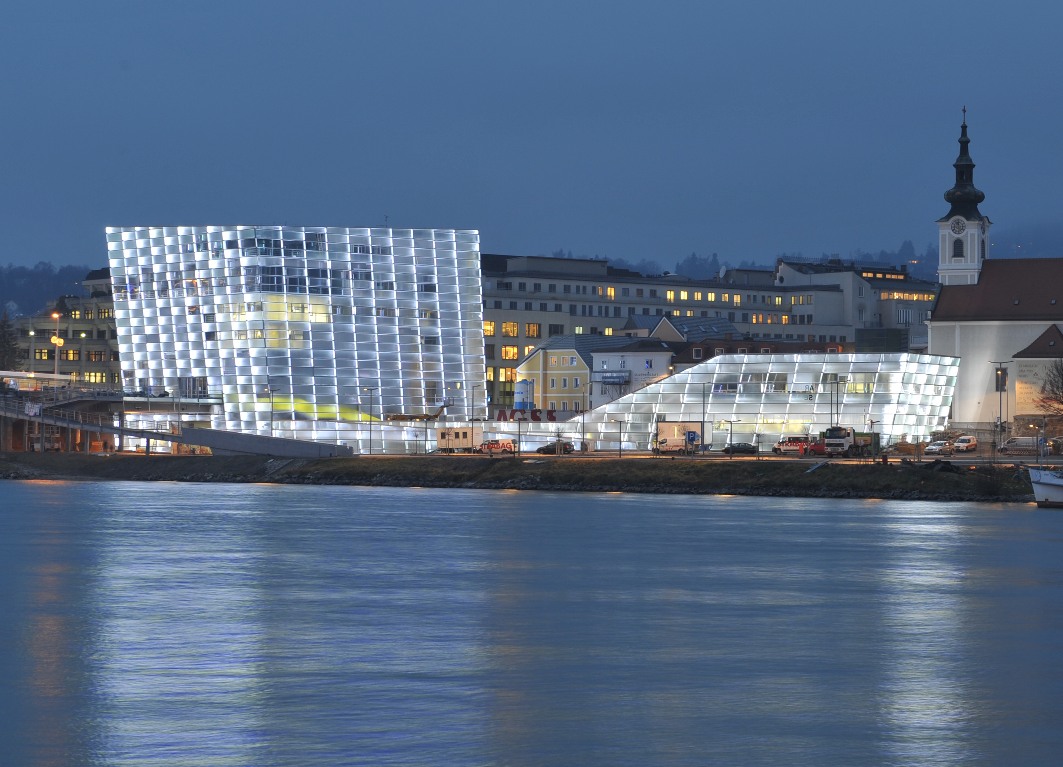
\includegraphics[width=8cm]{exFig.pdf}
% Below the figure, a caption is put, and a label is defined
% to be used for reference to this specific figure.
% Use labels which are very unlikely to be used by
% other contributors; for example, use labels starting
% with the surname of the first author.
\caption{\label{SchnabelTorrettaWesthues:fig1} (A) Plot of LD decay for Chromosome 1. (B) Sample of 
data with threshold and $\Delta_{0.5}$ indication. (C) Collection of $\Delta_{0.5}$ for Chromosome 1. 
(D) Smooth fit with indication of the the centromere.}
\end{figure}


% In the text, reference to the Figure can be made as follows:
%We refer to Figure~\ref{SchnabelTorrettaWesthues:fig1} for a~graphical representation.


%***********************************************************************

% Acknowledgments, if needed:
\acknowledgments{This case study was performed while the first and third author were 
visiting at Biometris at Wageningen University and Research Centre in winter 2014/2015. We are indebted to the group of Prof. Dr. Ruedi Fries, from Technische Universit\"at M\"unchen, for the SNP genotyping of the parental lines, which was funded by the German Federal Ministry of Education and Research (BMBF)  within the AgroClustEr “Synbreed—Synergistic plant and animal breeding” (FKZ:0315528d).}

%***********************************************************************

% References should be placed in the text in author (year) form.
% The list of references should be placed below IN ALPHABETICAL ORDER.
% (Please follow the format of the examples very tightly).

\references
%\begin{description}
%\item[Diggle, P.J., Liang, K-Y., and Zeger, S.L.] (1994).
%     {\it Analysis of Longitudinal Data}.
%     Oxford: Clarendon Press.
%\item[Green, P.J. and Silverman, B.W.] (1994).
%     {\it Nonparametric Regression and Generalized Linear Models}.
%     London: Chapman \& Hall.
%\item[Henderson, C.R.] (1973).
%     Sire evaluation and genetic trends.
%     In: {\it Proceedings of the Animal Breeding and Genetics Symposium in
%     Honour of Dr.\ L.\ Lush}, Champaign, Illinois, 10\,--\,41.
%\item[Lee, Y. and Nelder, J.A.] (1996).
%     Hierarchical generalized linear models.
%     {\it Journal of the Royal Statistical Society, Series B}, {\bf 58},
%      619\,--\,678.
%\item[Robinson, G.K.] (1991).
%     That BLUP is a good thing: the estimation of random effects (with Discussion).
%     {\it Statistical Science}, {\bf 6}, 15\,--\,51.
%\end{description}

\end{document}
